% Week 05 slides: version control with git and GitHub.
%
% Compile with XeLaTeX, not pdfLaTeX: the fonts are loaded with fontspec.
%
% In Positron, LaTeX Workshop's build button uses the "latexmk (XeLaTeX)" recipe
% in .vscode/settings.json. From a terminal, the same command is:
%
%     latexmk -xelatex -auxdir=.latex-build -outdir=. 05-git.tex
%
% Auxiliary files go in .latex-build/, which is gitignored. Only this file and
% 05-git.pdf are committed.

\documentclass[aspectratio=169,11pt]{beamer}

\usetheme[progressbar=frametitle, numbering=fraction]{metropolis}
\usepackage{amssymb}
\usepackage{pifont}

% Load Fira Mono by file name: XeLaTeX on Windows does not always find it by
% its font name, and falls back to a slanted substitute.
\setmonofont{FiraMono}[Extension=.otf, UprightFont=*-Regular, BoldFont=*-Bold, Scale=0.92]
\usepackage{tikz}
\usetikzlibrary{arrows.meta, positioning, fit}

% ---------------------------------------------------------------------------
% Colors: the course palette, taken from the "Your turn" box in the notebooks
% ---------------------------------------------------------------------------
\definecolor{ban}{HTML}{31708F}
\definecolor{banlight}{HTML}{D9EDF7}
\definecolor{good}{HTML}{3C763D}
\definecolor{bad}{HTML}{A94442}
\definecolor{softgray}{HTML}{6C757D}

\setbeamercolor{frametitle}{bg=ban, fg=white}
\setbeamercolor{progress bar}{fg=banlight, bg=ban!60}
\setbeamercolor{title separator}{fg=ban}
\setbeamercolor{alerted text}{fg=bad}
\setbeamercolor{block title}{bg=banlight, fg=ban}
\setbeamercolor{block body}{bg=banlight!40}

% Inline code and a highlighted keyword
\newcommand{\code}[1]{\texttt{#1}}
\newcommand{\key}[1]{\textbf{\textcolor{ban}{#1}}}
\newcommand{\ui}[1]{\textbf{#1}}

% The label above an exercise slide's title
\newcommand{\exerciseframe}[3]{%
  \begin{frame}[t]{#1}
    \vspace{0.4em}
    {\small\textcolor{softgray}{\textsc{exercise}}}\par\vspace{0.6em}
    #2
    \vfill
    \begin{block}{Steps}
      All steps and checks are in \key{exercises.md}. #3
    \end{block}
    \vspace{0.6em}
  \end{frame}}

\title{Version control with git and GitHub}
\subtitle{Week 05 workshop}
\author{BAN405 Python Programming for Data Science}
\date{}

\begin{document}

\maketitle

% ===========================================================================
\section{Why}
% ===========================================================================

\begin{frame}{A familiar problem}
  \begin{columns}[T]
    \begin{column}{0.45\textwidth}
      \ttfamily\small
      convert.py\\
      convert\_v2.py\\
      convert\_v2\_fixed.py\\
      convert\_final.py\\
      convert\_final\_v3\_ACTUAL.py
    \end{column}
    \begin{column}{0.52\textwidth}
      \begin{itemize}
        \item It worked yesterday. Today it does not.
        \item Which file is the one that worked?
        \item What changed between them, and why?
      \end{itemize}
      \vspace{1em}
      Every programmer has a folder like this. \key{Version control} is the fix.
    \end{column}
  \end{columns}
\end{frame}

\begin{frame}{Why not just OneDrive?}
  \begin{columns}[T]
    \begin{column}{0.48\textwidth}
      \textbf{A sync service} keeps
      \begin{itemize}
        \item the \emph{latest} state of every file
        \item older versions by \emph{time}, saved whenever it felt like it
        \item nothing about \emph{what} changed or \emph{why}
      \end{itemize}
    \end{column}
    \begin{column}{0.48\textwidth}
      \textbf{git} keeps
      \begin{itemize}
        \item snapshots \emph{you} decide to take
        \item each with a message saying \emph{why}
        \item and the exact lines that changed
      \end{itemize}
    \end{column}
  \end{columns}
  \vspace{1.5em}
  \centering
  A backup answers \emph{``can I get my file back?''}\\
  Version control also answers \emph{``what changed, when, and why?''}
\end{frame}

\begin{frame}{git and GitHub are two different things}
  \centering
  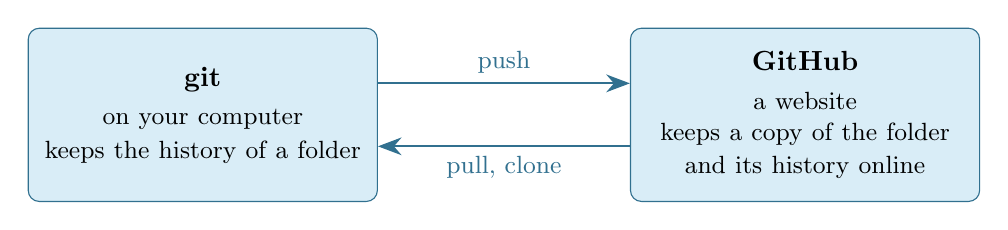
\begin{tikzpicture}[
      box/.style={draw=ban, fill=banlight, rounded corners, minimum width=4.4cm,
                  minimum height=2.2cm, align=center, text width=4.2cm},
      arr/.style={-{Stealth[length=3mm]}, thick, ban}]
    \node[box] (local) {\textbf{git}\\[0.3em]\small on your computer\\keeps the history of a folder};
    \node[box, right=3.2cm of local] (hub) {\textbf{GitHub}\\[0.3em]\small a website\\keeps a copy of the folder\\and its history online};
    \draw[arr] ([yshift=4mm]local.east) -- node[above]{\small push} ([yshift=4mm]hub.west);
    \draw[arr] ([yshift=-4mm]hub.west) -- node[below]{\small pull, clone} ([yshift=-4mm]local.east);
  \end{tikzpicture}

  \vspace{1.2em}
  \raggedright
  \begin{itemize}
    \item A \key{repository} is a folder whose history git keeps.
    \item A \key{commit} is one snapshot in that history.
  \end{itemize}
\end{frame}

\begin{frame}{What an analyst gets out of it}
  \begin{enumerate}
    \item \textbf{Explain what changed.} \emph{``The report said 12.4\,\% last week, and 11.9\,\% now. Why?''}
    \item \textbf{A backup}, and the same project on more than one computer.
    \item \textbf{Something to share}: a link instead of an email attachment, and a portfolio.
    \item \textbf{Working together} on one project without emailing files back and forth.
  \end{enumerate}
  \vspace{1em}
  git is the standard tool for all four, in software and in data teams alike.
\end{frame}

\begin{frame}{Today}
  Five exercises. Each adds \emph{one} new thing you can do.
  \vspace{0.8em}

  \centering
  \begin{tabular}{c l l}
    & \textbf{New skill} & \textbf{Where} \\ \hline
    1 & Read a history & on github.com \\
    2 & Clone and commit & a copy of someone else's project \\
    3 & Start a repository & your own BAN405 folder \\
    4 & Push & your BAN405 folder $\rightarrow$ GitHub \\
    5 & Pull & your repository on two computers \\
  \end{tabular}

  \vspace{1em}
  \raggedright
  Everything happens in Positron's \ui{Source Control} panel.\\
  Explanations, options and fixes are in the \key{git guide}, in the \code{guides} folder.
\end{frame}

% ===========================================================================
\section{Reading a history}
% ===========================================================================

\exerciseframe{Exercise 1 --- Read a history}{%
  \begin{itemize}
    \item A repository on GitHub holds the temperature converter you wrote yourself, in six commits.
    \item Look through the commits and their diffs.
    \item Then find the commit that made \code{212} °F come out as \code{85.8} °C.
  \end{itemize}}{You only need a browser.}

\begin{frame}{What you just saw}
  \begin{itemize}
    \item A \key{commit}: a message, an author, a date, and a \key{hash} such as \code{4803c4f}.
    \item A \key{diff}: the lines that changed. \textcolor{bad}{Red} removed, \textcolor{good}{green} added.
  \end{itemize}
  \vspace{0.8em}
  \begin{block}{The lesson}
    The commit was called \emph{``Tidy up formatting''}. It also changed the formula.\\[0.3em]
    The \textbf{message} is what someone meant to do. The \textbf{diff} is what they did.
  \end{block}
  \vspace{0.5em}
  Without the history you would be re-reading the whole program. With it, the answer is one click away.
\end{frame}

% ===========================================================================
\section{Making commits}
% ===========================================================================

\begin{frame}{The three places a change can be}
  \centering
  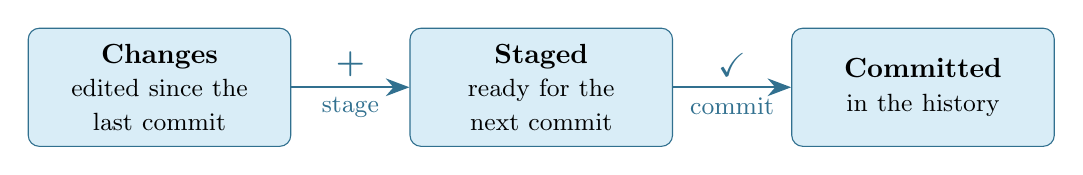
\begin{tikzpicture}[
      box/.style={draw=ban, fill=banlight, rounded corners, text width=3.1cm,
                  minimum height=1.5cm, align=center},
      arr/.style={-{Stealth[length=3mm]}, thick, ban}]
    \node[box] (changes) {\textbf{Changes}\\\small edited since the last commit};
    \node[box, right=1.5cm of changes] (staged) {\textbf{Staged}\\\small ready for the next commit};
    \node[box, right=1.5cm of staged] (committed) {\textbf{Committed}\\\small in the history};
    \draw[arr] (changes) -- node[above]{\large\bfseries +} node[below]{\small stage} (staged);
    \draw[arr] (staged) -- node[above]{\large$\checkmark$} node[below]{\small commit} (committed);
  \end{tikzpicture}

  \vspace{1.2em}
  \raggedright
  \begin{itemize}
    \item \textbf{Staging} lets you choose what goes into a commit, instead of everything at once.
    \item \textbf{Discard Changes} throws away everything since your last commit. It is the undo you will use most.
  \end{itemize}
\end{frame}

\begin{frame}{Not everything belongs in the history}
  \begin{columns}[T]
    \begin{column}{0.5\textwidth}
      A \key{\code{.gitignore}} is a text file listing what git should never track.
      \vspace{0.6em}

      \textbf{Keep out}
      \begin{itemize}
        \item files your computer makes by itself\\\small(\code{\_\_pycache\_\_}, \code{.DS\_Store})
        \item files your code produces\\\small(figures, tables)
        \item \alert{secrets}: passwords and keys
        \item \alert{personal data} about other people
      \end{itemize}
    \end{column}
    \begin{column}{0.46\textwidth}
      \begin{block}{The rule}
        Every new repository starts with the course template:\\[0.3em]
        \code{guides/gitignore-template.txt}\\[0.3em]
        Copy it into \code{.gitignore}, and commit it first.
      \end{block}
      \vspace{0.4em}
      \small Once something is pushed, assume it is public, even in a private repository. Deleting it later leaves it in the history.
    \end{column}
  \end{columns}
\end{frame}

\exerciseframe{Exercise 2 --- Clone it and fix it}{%
  \begin{itemize}
    \item \textbf{Together:} tell git who you are (the \emph{one} terminal step today), and clone the temperature converter into a \code{git-practice} folder.
    \item \textbf{On your own:} keep a secret out of git with a \code{.gitignore}, fix the bug, and commit both.
    \item Break something on purpose, and undo it.
  \end{itemize}}{Mac: \textbf{Terminal}. Windows: \textbf{Git Bash}.}

\begin{frame}{Good commits}
  \begin{itemize}
    \item \textbf{Commit when you finish something}, not when you are happy with everything.
    \item \textbf{One commit, one change.} A fix and a new feature are two commits.
    \item \textbf{Write the message for whoever reads the history next.} Usually you.
  \end{itemize}
  \vspace{0.6em}
  \centering
  \begin{tabular}{l l}
    \textcolor{bad}{\ding{55}}\ \code{fix stuff} & \textcolor{good}{$\checkmark$}\ \code{Fix crash when the input is empty} \\
    \textcolor{bad}{\ding{55}}\ \code{update}    & \textcolor{good}{$\checkmark$}\ \code{Add absolute-zero check to the converter} \\
    \textcolor{bad}{\ding{55}}\ \code{final}     & \textcolor{good}{$\checkmark$}\ \code{Split the analysis into functions} \\
  \end{tabular}
\end{frame}

% ===========================================================================
\section{Your own repository}
% ===========================================================================

\begin{frame}{Where the history lives: \code{.git}}
  \begin{columns}[T]
    \begin{column}{0.44\textwidth}
      \ttfamily\small
      \textcolor{softgray}{git-practice/}\\
      └── temperature-converter/\\
      \ \ \ \ ├── \textbf{.git/}\ \ \textcolor{ban}{$\leftarrow$ the history}\\
      \ \ \ \ ├── .env\ \ \ \ \ \ \textcolor{ban}{$\leftarrow$ ignored}\\
      \ \ \ \ ├── .gitignore\\
      \ \ \ \ ├── convert.py\\
      \ \ \ \ ├── README.md\\
      \ \ \ \ └── temperature\_tools.py
    \end{column}
    \begin{column}{0.52\textwidth}
      \begin{itemize}
        \item A \key{repository} is a folder plus its hidden \code{.git} folder: the whole history.
        \item Names starting with a dot are hidden by default.
        \item Delete \code{.git}, and git forgets the history. Your files stay.
      \end{itemize}
      \vspace{0.2em}
      \begin{block}{Together: show hidden files}
        \textbf{Windows:} File Explorer $\rightarrow$ \ui{View} $\rightarrow$ \ui{Show} $\rightarrow$ \ui{Hidden items}\\
        \textbf{Mac:} in Finder, press \code{Cmd+Shift+.}
      \end{block}
    \end{column}
  \end{columns}
\end{frame}

\begin{frame}{One repository: your whole BAN405 folder}
  \begin{columns}[T]
    \begin{column}{0.44\textwidth}
      \ttfamily\small
      \textcolor{softgray}{your computer}\\
      ├── \textbf{BAN405/}\ \ \textcolor{ban}{$\leftarrow$ repository}\\
      │\ \ \ ├── .gitignore\\
      │\ \ \ ├── data/\\
      │\ \ \ ├── week01/\\
      │\ \ \ └── ...\\
      └── git-practice/\ \ \textcolor{ban}{$\leftarrow$ clones}
    \end{column}
    \begin{column}{0.52\textwidth}
      \begin{enumerate}
        \item \textbf{Initialize once}, in the BAN405 folder itself.
        \item \textbf{Never} start a repository inside one of its folders.
        \item \textbf{Always open the BAN405 folder} in Positron, not a week folder.
        \item \textbf{Clone other projects next to it}, never inside it.
      \end{enumerate}
    \end{column}
  \end{columns}
\end{frame}

\exerciseframe{Exercise 3 --- Start your own repository}{%
  \begin{itemize}
    \item Open your BAN405 folder in Positron, and initialize a repository.
    \item Add the \code{.gitignore} template.
    \item Make your first commit.
  \end{itemize}}{}

% ===========================================================================
\section{GitHub}
% ===========================================================================

\begin{frame}{Push: give your history a copy online}
  \begin{itemize}
    \item \key{Push} sends your commits to GitHub. Until then, they exist only on your computer.
    \item \key{Private} repositories are visible only to you. \key{Public} ones, to anyone.
    \item Positron signs you in to GitHub through your browser: no passwords in a terminal.
  \end{itemize}
  \vspace{0.6em}
  \begin{block}{Positron's words for it}
    \begin{tabular}{@{}l l@{}}
      \ui{Publish Branch} & create the repository on GitHub, then push \\
      \ui{Sync Changes}   & pull, then push \\
    \end{tabular}
  \end{block}
\end{frame}

\exerciseframe{Exercise 4 --- Put it on GitHub}{%
  \begin{itemize}
    \item Publish your BAN405 repository as a \textbf{private} repository.
    \item Add a README, commit it, and push.
    \item Look at the result on github.com.
  \end{itemize}}{}

\begin{frame}{Two copies of one repository}
  \centering
  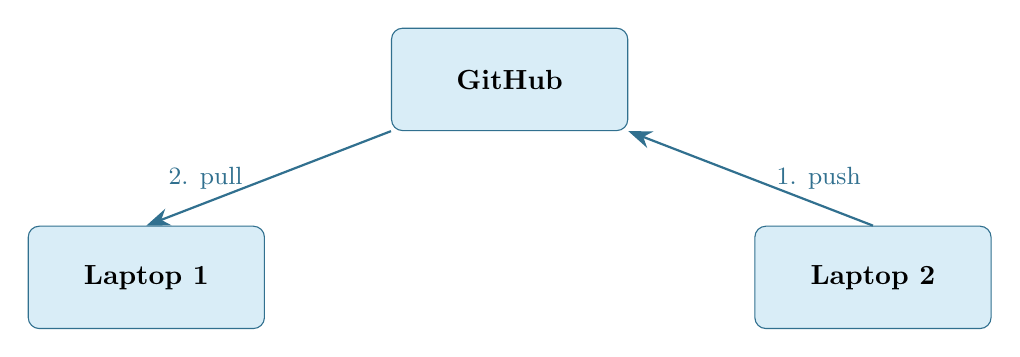
\begin{tikzpicture}[
      box/.style={draw=ban, fill=banlight, rounded corners, minimum width=3cm,
                  minimum height=1.3cm, align=center},
      arr/.style={-{Stealth[length=3mm]}, thick, ban}]
    \node[box] (hub) {\textbf{GitHub}};
    \node[box, below left=1.2cm and 1.6cm of hub] (one) {\textbf{Laptop 1}};
    \node[box, below right=1.2cm and 1.6cm of hub] (two) {\textbf{Laptop 2}};
    \draw[arr] (two.north) -- node[right, xshift=2mm]{\small 1. push} (hub.south east);
    \draw[arr] (hub.south west) -- node[left, xshift=-2mm]{\small 2. pull} (one.north);
  \end{tikzpicture}

  \vspace{1em}
  \raggedright
  Copies do not update each other. Two habits keep them in step:
  \begin{itemize}
    \item \key{Pull} when you start working.
    \item \key{Push} when you finish, even if the work is unfinished.
  \end{itemize}
\end{frame}

\exerciseframe{Exercise 5 --- Work from a second computer}{%
  \begin{itemize}
    \item You have one computer here, so \textbf{github.com stands in for the second}: an edit there is a commit your computer has not seen, just like a push from your other laptop.
    \item Edit the README on github.com, then \key{pull} it into Positron.
    \item \emph{Optional:} forget to pull, and see what happens.
  \end{itemize}}{Editing on github.com is only a stand-in: in your own work, change files on your computer and push.}

% ===========================================================================
\section{When copies disagree}
% ===========================================================================

\begin{frame}{Merge conflicts}
  A conflict needs \textbf{two copies that both changed the same lines}: \textbf{you on two computers}, or \textbf{two people} in one repository. git will not guess which version is right, so it marks the spot and asks you.
  \vspace{0.8em}
  \begin{columns}[T]
    \begin{column}{0.5\textwidth}
      \textbf{Avoiding them}
      \begin{enumerate}
        \item Pull when you start, push when you finish.
        \item Commit small and often.
        \item Divide the work by file.
        \item One person per notebook. Always.
      \end{enumerate}
    \end{column}
    \begin{column}{0.46\textwidth}
      \textbf{Notebooks} store their output as well as their code. Never merge one by hand: keep \emph{one} whole version, and redo the other change.
    \end{column}
  \end{columns}
\end{frame}

\begin{frame}[t]{Demo: forgetting to pull}
  \vspace{0.3em}
  {\small\textcolor{softgray}{\textsc{live demo}}}\par\vspace{0.4em}
  \begin{enumerate}
    \item \textbf{On the other computer} {\small\textcolor{softgray}{(github.com stands in)}}: change a line of \code{README.md}, and commit.
    \item \textbf{On this computer, without pulling}: change the \emph{same} line differently. Stage, commit.
    \item \ui{Sync Changes}. git pulls first --- and stops. \code{README.md} is listed under \ui{Merge Changes}.
  \end{enumerate}
  \vfill
  \begin{block}{Why}
    Both copies changed the same line since they were last in step. git will not guess which one is right, so it asks you.
  \end{block}
\end{frame}

\begin{frame}[t]{Demo: resolving the conflict}
  \vspace{0.3em}
  {\small\textcolor{softgray}{\textsc{live demo}}}\par\vspace{0.4em}
  \begin{columns}[T]
    \begin{column}{0.46\textwidth}
      git marks the spot in the file:
      \vspace{0.4em}

      {\ttfamily\footnotesize
      \textcolor{bad}{<{}<{}<{}<{}<{}<{}< HEAD}\\
      My work, edited on this computer.\\
      \textcolor{bad}{=======}\\
      My work, edited on the other one.\\
      \textcolor{bad}{>{}>{}>{}>{}>{}>{}> 7bdf541...}\par}
      \vspace{0.6em}
      {\small \emph{Current} is yours. \emph{Incoming} is what you pulled.}
    \end{column}
    \begin{column}{0.5\textwidth}
      \begin{enumerate}
        \setcounter{enumi}{3}
        \item Choose \ui{Accept Current}, \ui{Accept Incoming} or \ui{Accept Both}, or edit by hand. No marker lines may remain.
        \item Save, stage with \ui{+}, and commit. The message is written for you.
        \item \ui{Sync Changes}. In Positron's \ui{Graph}, the two lines of history join in a \key{merge commit}.
      \end{enumerate}
    \end{column}
  \end{columns}
\end{frame}

% ===========================================================================
\section{From now on}
% ===========================================================================

\begin{frame}{The habit to keep}
  \begin{center}
    \Large Commit as you work.\quad Push when you finish.
  \end{center}
  \vspace{1em}
  \begin{itemize}
    \item Your BAN405 repository is where your work for the rest of the course lives.
    \item Pull when you start, if you use more than one computer.
    \item When something goes wrong: the \key{git guide}, section \emph{Troubleshooting}.
  \end{itemize}
\end{frame}

\begin{frame}{What we did not cover}
  Today was the basics. Worth knowing these exist, and the git guide covers each:
  \begin{itemize}
    \item \key{Fork}: a copy of someone else's repository in \emph{your} GitHub account. A clone lives on your computer; a fork lives on GitHub.
    \item \key{Pull request}: asking a repository's owner to accept your changes. How open-source software is built.
    \item \key{Branches}: parallel lines of history, so a team can work on several things at once.
    \item \key{Template}: a new repository starting from someone else's files, with no history.
    \item \key{git in the terminal}: everything you did today, typed. Most tutorials use it.
  \end{itemize}
\end{frame}

\begin{frame}[t]{What you did today}
  \begin{columns}[T]
    \begin{column}{0.52\textwidth}
      \textbf{Today you}
      \small
      \begin{itemize}
        \item found a bug by reading a history
        \item cloned a project and committed a fix
        \item kept a secret out with \code{.gitignore}
        \item put your BAN405 folder on GitHub
        \item kept two computers in step
      \end{itemize}
    \end{column}
    \begin{column}{0.44\textwidth}
      \textbf{At home} {\small (in \key{exercises.md})}
      \small
      \begin{itemize}
        \item Commit your earlier work, one exercise per commit.
        \item \emph{Optional:} cause a merge conflict with a classmate.
      \end{itemize}
    \end{column}
  \end{columns}
  \vfill
  \begin{block}{Next week}
    The terminal, paths and conda: where your files really are, and how to make a project run on someone else's computer.
  \end{block}
\end{frame}

\end{document}
